\documentclass[11pt]{article}
\usepackage[T1]{fontenc}
\usepackage[utf8]{inputenc}
\usepackage{times}
\usepackage{eurosym}
\usepackage{inconsolata}
\usepackage{amsmath}
\usepackage{framed}
\usepackage{graphicx}
\usepackage{hyperref}
\hypersetup{colorlinks=true, linkcolor=blue, urlcolor=blue}
\usepackage[usenames,dvipsnames,svgnames,table]{xcolor}
\definecolor{entityColor}{RGB}{0,100,200}
\definecolor{attributeColor}{RGB}{0,100,50}
\definecolor{relationColor}{RGB}{160,0,30}
\usepackage{listings}
\lstdefinestyle{reqT}{
  belowcaptionskip=1\baselineskip,
  breaklines=true,
  showstringspaces=false,
  basicstyle=\footnotesize\ttfamily,
  emph={Ent,Meta,Item,Label,Section,Term,Actor,App,Component,Domain,Module,Product,Release,Resource,Risk,Service,Stakeholder,System,User,Class,Data,Input,Member,Output,Relationship,Design,Screen,MockUp,Function,Interface,Epic,Feature,Goal,Idea,Issue,Req,Ticket,WorkPackage,Breakpoint,Barrier,Quality,Target,Scenario,Task,Test,Story,UseCase,VariationPoint,Variant},
  emphstyle=\bfseries\color{entityColor},
  emph={[2]has,is,superOf,binds,deprecates,excludes,helps,hurts,impacts,implements,interactsWith,precedes,requires,relatesTo,verifies},
  emphstyle={[2]\bfseries\color{relationColor}},
  emph={[3]Attr,Code,Constraints,Comment,Deprecated,Example,Expectation,FileName,Gist,Image,Spec,Text,Title,Why,Benefit,Capacity,Cost,Damage,Frequency,Min,Max,Order,Prio,Probability,Profit,Value,Status},
  emphstyle={[3]\color{attributeColor}},  
}
\lstset{style=reqT}
\usepackage{fancyvrb}
\usepackage[english]{babel}
\usepackage{blindtext}
\usepackage{enumitem} 
\setlist[itemize]{noitemsep}
\title{{\bf LAB 2:\\Requirements Prioritization \& Release Planning}\\ Instructions
}
\author{Björn Regnell}
\date{\today}
\begin{document}
\maketitle

\section{Introduction}

\subsection{Purpose} This document provides instructions on how to run 
a computer lab session on requirements prioritization and release planning with computer tools, and demonstrates the complexity in finding solutions to these problems.  

\subsection{Prerequisites} This lab assumes that you have installed the open source tool \href{http://reqT.org}{reqT.org} and that you are familiar with basic requirements modeling using reqT. It is also assumed that you have completed \href{https://github.com/reqT/reqT/raw/3.0.x/doc/lab1/lab1.pdf}{Lab 1 Requirements Modeling}. You should also complete the preparations for Lab 2, available at \url{https://github.com/reqT/reqT/raw/3.0.x/doc/lab2/lab2.pdf} 

You should bring a file \verb+prio100.scala+ from the Lab 2 preparations to the lab computer. The file should include a reqT scala Model with at least two Stakeholder entities, each with a Prio attribute and a set of at least 15 Req entities each with a Benefit attribute. The integer Prio values should reflect the importance of each Stakeholder and the Benefit values should include your results from a \$100-method prioritization session.  


\clearpage\newpage
\section{Instructions}\label{section:instr}

\subsection{Prioritization}


\subsubsection{Ratio scale prioritization}
In this section you will use reqT to calculate resulting priorities based on input from your \$100-method priority session. 
\begin{framed}
\noindent Do the following steps: 

\begin{enumerate}
\item Load your \verb+prio100.scala+ model into the tree in the reqT ModelTreeEditor.
\item Enter the following code in the reqT text editor. Similar code is available in the menu item:  Templates -> Prioritization \$100 Method.
\begin{lstlisting}
m =>    
val shs = m.entitiesOfType(Stakeholder)
val rs = m.entitiesOfType(Req)
val prioSum = shs.map(s => m/s/Prio).sum
val benefitSum = shs.map(s => 
  s -> (m/s).collect{ case Benefit(b) => b}.sum).toMap
val normalized = rs.map(r => 
  r has Benefit(
    math.round(shs.map(s => 
      (m/s/Prio)*(m/s/r/Benefit)*100.0 / (benefitSum(s)*prioSum)).sum).toInt)).toModel
println("\n--- Normalized, weighted priorities:\n" + normalized)
val sum = normalized.collect{ case Benefit(b) => b}.sum
println("\n--- Sum: " + sum)
println(normalized)
normalized.toString.save("prio100-result.scala")
m 
\end{lstlisting}
\item Apply the above function to the tree containing your prio100 model. Check the console for output.
\item What 5 requirements have the highest total normalized priority?
\vspace{4em}
\item Change the priorities of the stakeholders. How did the normalized requirements benefit change?
\vspace{4em}
\item Use a web browser to navigate to the reqT source code at GitHub and in the source file in \verb+src/reqT+ named \verb+ModelBasicOps.scala+ search for ''\verb+def entitiesOfType+'' and explain what that method does. \newline a) What is the result type? \vspace{1em}\newline b) Can the collection include duplicate items? (Hint: search for ''\verb+lazy val entities+'' and check if the method \verb+distinct+ is applied or not.)
\vspace{1em}
\item Check the code ins step 2 above and match each code line with the calculations in the preparations Section 2.1.2. Explain to a friend what the code above does. You can insert \verb+println+ of interesting values to better understand what the contain, e.g. \verb+println(benefitSum)+. Write down which {\verb+val+} declarations in the above code that correspond to which sums in the formulas in the preparations? 
\vspace{6em}
\item Open a spread sheet program (e.g. LibreOffice Calc or MS Excel) and create the column headings Stakeholder;Feature;Prio and fill in the columns similar to this, using your own priorities:
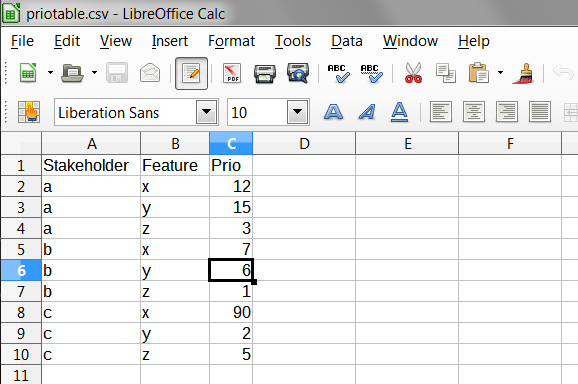
\includegraphics[width=0.9\textwidth]{spread-sheet.png}
\item Use Save As ... or Export and save your spread sheet in the .csv text file format, using semicolons as column separators (the default is depending on your locale). Open the file in a text editor and check that it has semicolons as column separators. Fix it if not, e.g. using your favorite editor's search-replace feature.
\item Select the Import -> From Prio Table menu item in the reqT gui, and import your spread sheet to the tree.
\item Add a Prio attribute to each stakeholder in the tree, using <Ctrl+E> and <Ctrl+R>, to model that stakeholders have different importance.
\item Calculate the normalized total priorities using the code from step 2 above. The code might be available in your undo history, check with <Ctrl+Z> in the text editor pane of the reqT gui.
\item Discuss with a friend how you could use the Import -> From Prio Table feature of reqT when you elicit priorities in your project. How would you prepare the data collection from stakeholders?
\item Extra if you are curious: Investigate the code in the reqT source file named \verb+parse.scala+ in the reqT repo at GitHub. How could you use the \verb+load+ method in \verb+ object Tab + to import a .csv file that have another character than semicolon as column separator? 
\end{enumerate}

\end{framed}

\subsubsection{Ordinal scale prioritization}
\blindtext


\clearpage\newpage 

\subsection{Release Planning}
\blindtext
\subsubsection{Without coupling and precedence constraints}
\blindtext
\subsubsection{With coupling and precedence constraints}
\blindtext
\end{document}
